\section{Comparing Exclusion Limits - both between ML models and previous analysis}
In the previous section I compared the achieved significance between 
the three optimal models for the full statistics signal set. In this section 
I will do the same, but with the introduction of a $20\%$ uncertainty in the background.
Additionally, I will compare the achieved exclusion limits (the mass combinations with an achieved 
significance of over 1.64) by the models created in this thesis, with the limit set in the paper (INSERT 
HERE).

\begin{figure}
    \makebox[\linewidth][c]{%
    \centering
    \begin{subfigure}{.85\textwidth}
        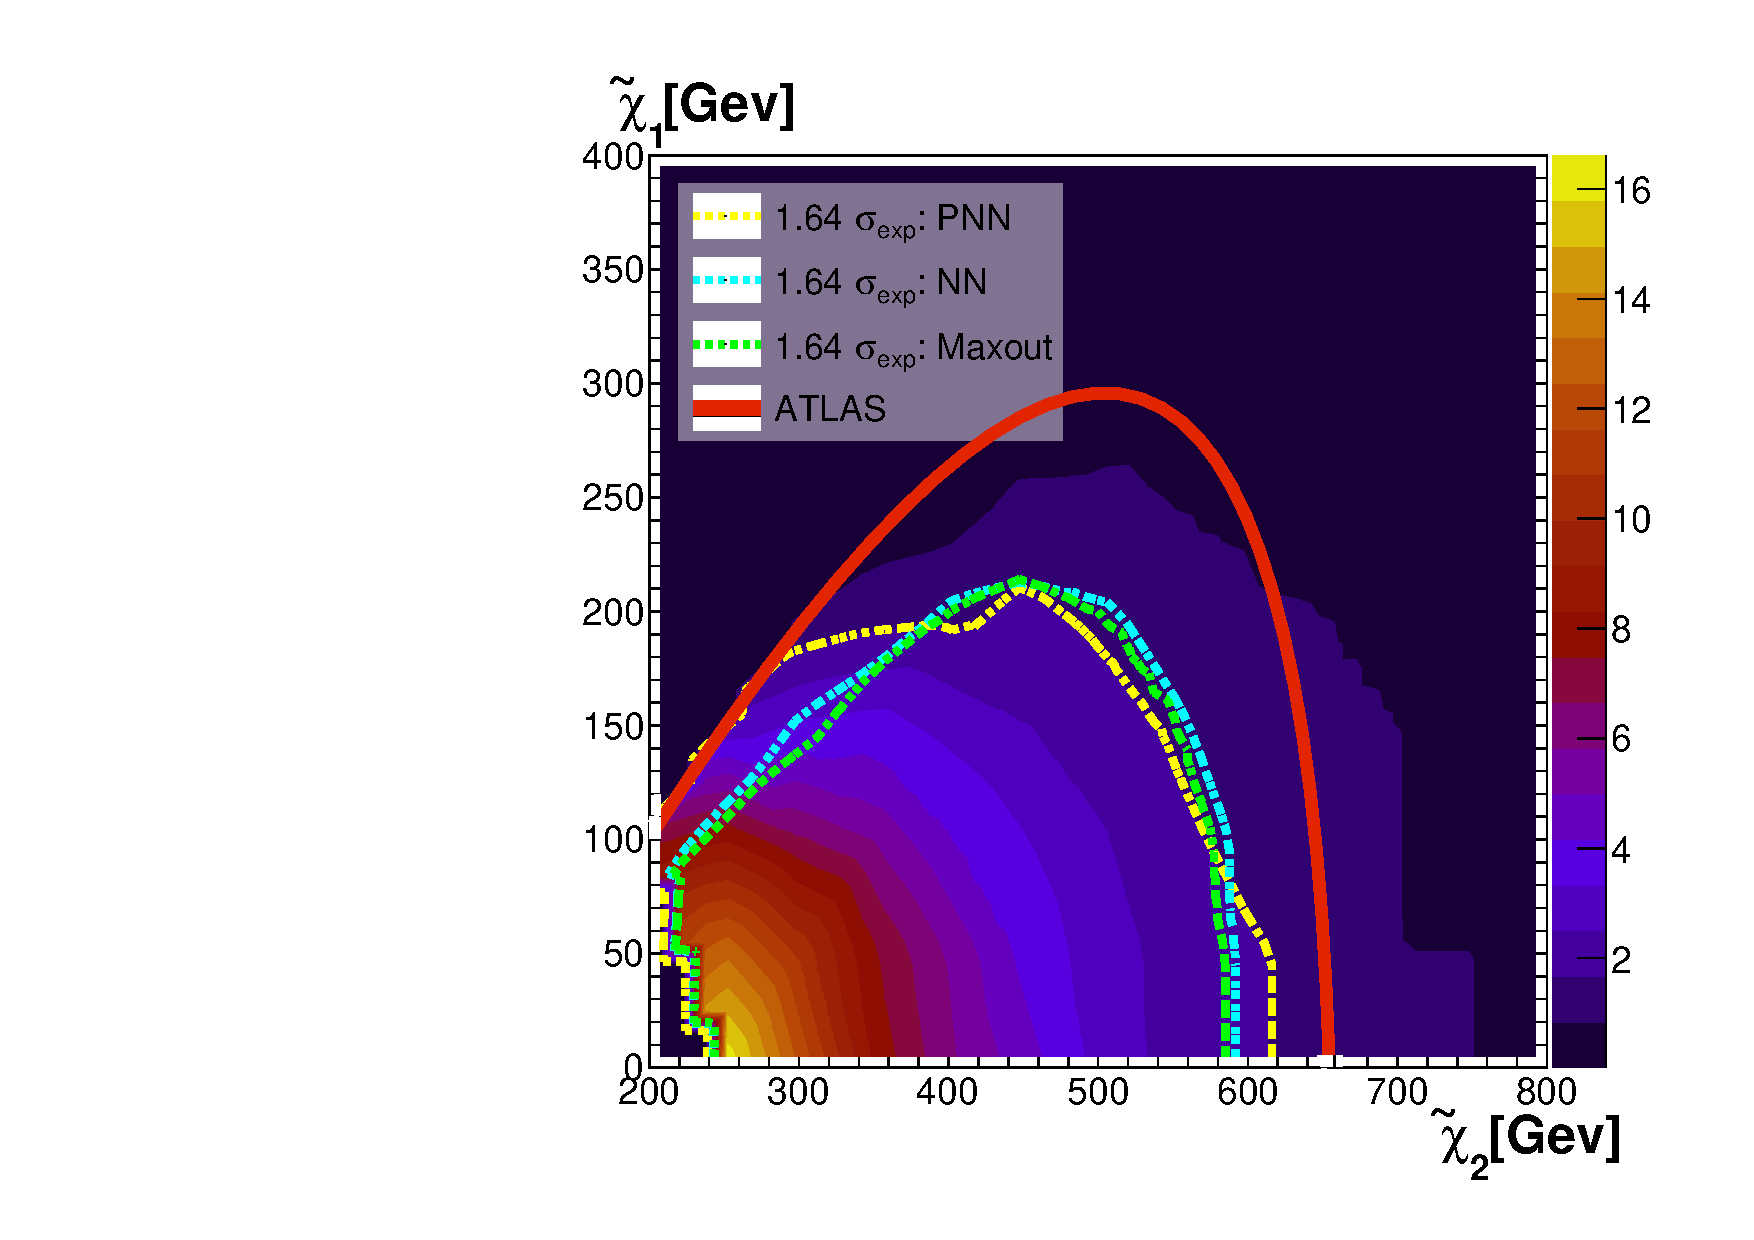
\includegraphics[width=\textwidth]{Figures/MLResults/NN/SUSY/Comparison/compLimitEdit.pdf}
    \end{subfigure}
    }
    \caption{A grid displaying the achieved significance on the full statistics signal set, using the signal region 
    created by the \emph{PNN} network.}
    \label{fig:compLimit}
\end{figure}